%; whizzy chapter
% -initex iniptex -latex platex -format platex -bibtex jbibtex -fmt fmt
% 以上 whizzytex を使用する場合の設定.

%     Kansai Debian Meeting resources
%     Copyright (C) 2007 Takaya Yamashita
%     Thank you for Tokyo Debian Meeting resources

%     This program is free software; you can redistribute it and/or modify
%     it under the terms of the GNU General Public License as published by
%     the Free Software Foundation; either version 2 of the License, or
%     (at your option) any later version.

%     This program is distributed in the hope that it will be useful,
%     but WITHOUT ANY WARRANTY; without even the implied warranty of
%     MERCHANTABILITY or FITNESS FOR A PARTICULAR PURPOSE.  See the
%     GNU General Public License for more details.

%     You should have received a copy of the GNU General Public License
%     along with this program; if not, write to the Free Software
%     Foundation, Inc., 51 Franklin St, Fifth Floor, Boston, MA  02110-1301 USA

%  preview (shell-command (concat "evince " (replace-regexp-in-string "tex$" "pdf"(buffer-file-name)) "&"))
% 画像ファイルを処理するためには ebb を利用して boundingbox を作成.
%(shell-command "cd image200708; ebb *.png")

%%ここからヘッダ開始.

\documentclass[mingoth,a4paper]{jsarticle}
\usepackage{kansaimonthlyreport}
\usepackage[dvips]{xy}
\usepackage{ascmac}

% 日付を定義する, 毎月変わります.
\newcommand{\debmtgyear}{2011}
\newcommand{\debmtgdate}{27}
\newcommand{\debmtgmonth}{02}
\newcommand{\debmtgnumber}{44}

\begin{document}

\begin{titlepage}

% 毎月変更する部分, 本文の末尾も修正することをわすれずに

 第\debmtgnumber{}回 関西 Debian 勉強会資料

\vspace{2cm}

\begin{center}
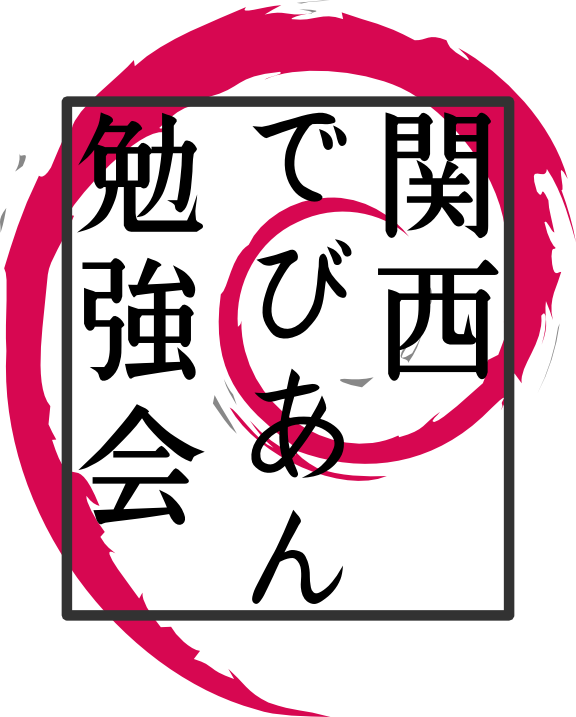
\includegraphics{image200802/kansaidebianlogo.png}
\end{center}

\begin{flushright}
\hfill{}関西 Debian 勉強会担当者 佐々木・倉敷・のがた \\
\hfill{}\debmtgyear{}年\debmtgmonth{}月\debmtgdate{}日
\end{flushright}

\thispagestyle{empty}
\end{titlepage}

\dancersection{Introduction}{Debian JP}

\subsection*{}%ロゴ用のスペース稼ぎ

関西 Debian 勉強会は Debian GNU/Linux のさまざまなトピック (新しいパッケー
ジ, Debian 特有の機能の仕組, Debian 界隈で起こった出来事, などなど) に
ついて話し合う会です.

目的として次の三つを考えています.
\begin{itemize}
      \item ML や掲示板ではなく, 直接顔を合わせる事での情報交換の促進
      \item 定期的に集まれる場所
      \item 資料の作成
\end{itemize}

それでは, 楽しい一時をお楽しみ下さい.

\clearpage

\begin{minipage}[b]{0.2\hsize}
 {\rotatebox{90}{\fontsize{80}{80}
{\gt 関西 Debian 勉強会}}}
\end{minipage}
\begin{minipage}[b]{0.8\hsize}
\hrule
\vspace{2mm}
\hrule
\setcounter{tocdepth}{1}
\tableofcontents
\vspace{2mm}
\hrule
\end{minipage}

\dancersection{最近の Debian 関係のイベント報告}{Debian JP}

\subsection{Squeezeがリリースされました}

\begin{wrapfigure}{l}{4.5cm}
  \begin{center}
   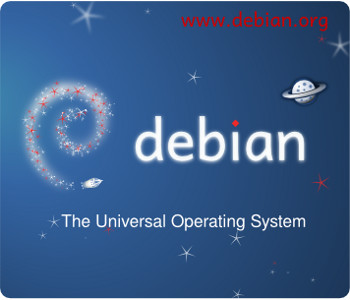
\includegraphics[width=4.5cm]{image201102/bannersqueeze.jpg}
  \end{center}
 \vspace{-0.5cm}
\end{wrapfigure}

カウントダウンバナーも用意され
\footnote{\url{http://news.debian.net/2011/01/22/join-us-in-the-countdown-to-squeeze/}}
、本当にカウントダウンどおりにリリースされるのか?と妙な心配もされた
Debian 6.0 Squeezeですが、2月6日に無事リリースされました。

なぜ2月6日に設定されたのかというと、ちょうどその時、FOSDEM(Free and Open
Source Development European Meeting)が開催されていて、それに合わせたみた
いです。

リリースの様子はidenti.ca(自由なソフトウェアでtwitterのようなマイクロブロ
ギングサービス)のDebianアカウント
\footnote{\url{http://identi.ca/debian}}でも中継され、identi.ca/twitter
で、かなり盛り上がっていました。

\subsection{第 43 回関西 Debian 勉強会}

1月23日、大阪港区民センターにて第43回関西Debian勉強会が開かれ、杉本さんに
よるDebian GNU/kFreeBSDについての発表「Debian GNU/kFreeBSDで便利に暮らす
ためのTips」と、のがたのバグ報告についての発表「バグ報告はバグのためだけ
じゃないよ」がありました。

杉本さんのkFreeBSDの発表は、常用できるとはいえ、細かなところではまだまだ
問題が残っているので、もっと骨があるやつをいじりたいぜ!という人には、もっ
てこいのプラットフォームですね。

のがたのバグレポートの話は、ブラッシュアップして、バグ報告の入門ぐらいに
はしたいですね。

\subsection{第 73 回東京エリア Debian 勉強会}

2月19日に行われた第73回東京エリアDebian勉強会では、HadoopとDebian Games
Team体験記、リリースされてばかりのSqueezeについて、みんなで話し合われたそ
うです。

Debian Games Teamで活動するきっかけとなったXmrisは、Mr. Doクローンなんで
すね。懐かしくてちょっとやってみたいなと思いました。
CAcertについても、まだ盛り上がっているようです。

\clearpage

%-------------------------------------------------------------------------------
\dancersection{事前課題}{Debian JP}

今回は以下の課題を設定しました.
%
\begin{quote}
    \begin{screen}
     ついに Squeeze がリリースされました。そんなわけで Squeeze になって
     \begin{itemize}
      \item よかったこと
      \item うれしかったこと
      \item (些細な事だけど)こんな所が変わった!
      \item いきなりナニカ踏んだ!!
     \end{itemize}
     なんて事柄を、なにか一つご報告下さい。
    \end{screen}
 \end{quote}
 %
 参加者の皆さんによる回答は以下の通りです.

\begin{prework}{ 甲斐正三 }
 シリアル通信(ttyUSB0)が一般ユーザーでは使えなくなってあせっています。
\end{prework}


\begin{prework}{ 山下康成 }
 rc が変わってはまりました。LSB ヘッダ必須とか、updaterc.d 必須とか、、
\end{prework}

\begin{prework}{ 八津尾 }
リリースされて本当によかった
\end{prework}

\begin{prework}{ 山下尊也 }
 \begin{itemize}
  \item よかったこと \\
        全体的にバージョンがあがったことで、比較的新しいソフトが動かせるようになりました。
        すいません。普段からsidなので、まったく思いつかなかったです...
 \end{itemize}
\end{prework}

\begin{prework}{ のがたじゅん }
 \begin{itemize}
  \item よかったこと \\
        デスクトップテーマのSpace Funがイカす!
        起動が早くなった。
        backportsが正式にDebianになったので新しいパッケージが欲しい人にbackportsを使ったら?と言いやすくなった。
  \item 残念だったこと \\
        Squeezeが残念、ではなく自分の取り組みで残念だったことですが
        SqueezeのDebian Liveに時間が取れなかった事が心残りです。Wheezey
        がんばります。
 \end{itemize}
\end{prework}

\begin{prework}{ 古川竜雄 (frkwtto@gmail.com) }
すいません。まだインストールしてません。ごめんなさい。
\end{prework}

\begin{prework}{ 川江 }
とにかく、リリース「おめでとう」です。25日1時55分の時点でまだ、AirにSqueezeをインストールできてませんが、日曜までになんとかインストールするつもりです。
\end{prework}

\begin{prework}{ 木下達也 }
 \begin{itemize}
  \item よかったこと:リリースされたこと
 \end{itemize}
\end{prework}

\begin{prework}{ 山田 洋平 }
dwm のバージョンが 4.7 から 5.8 に上がり、仕様も新しくなりました。
Wikipedia にも載っていますがステータスバーに表示する仕方が変わったりなど。
でも今見たらパッケージの説明文が古いままです。
バグ報告しなきゃですかねこれは。
\end{prework}

\begin{prework}{ 松澤二郎 }
 \begin{itemize}
  \item うれしかったこと:Space Funがすてき
 \end{itemize}
\end{prework}

\begin{prework}{ occult.zzz (立川勝宣) }

 \begin{itemize}
  \item よかった事 \\
        初めから二画面のドライバーが入っており使いやすかった。
        lenyの時は、ドライバーを探すのに入れすぎで
        何度もシステムを潰してしまい、結果それが、学ぶ一つになりました。
        やりはじめたばかりで、疑問多数なので、ぜひ参加させてください。
        よろしくお願い致します。
 \end{itemize}
\end{prework}

\begin{prework}{ 水野源 }
SheevaPlugでずっとtestingなsqueezeを使っていたので、正式リリースされて嬉しいです。
今回の発表資料を作る際にsqueezeのpbuilderでubuntu環境を作ろうとして、キーリングが自動で渡らないので構築に失敗する問題踏みましたょ。
\end{prework}

\begin{prework}{ かわだてつたろう }
 \begin{itemize}
  \item first point release が三月に予定されている
  \item dropbox が入らなかった
  \item nodejs が入らなかった
 \end{itemize}
\end{prework}

\begin{prework}{ lurdan }
何台か lenny からのアップグレードをしていますが、単機能サーバばかりなせいか、表紙抜けするくらいあっさりと完了しています。
dependency boot への移行がやたら失敗するくらいかな? 別に有り難くもないのでこれは気にしてません。
\end{prework}

\begin{prework}{ 中川舟(しゅう) }
 \begin{itemize}
  \item こんな所が変わった! \\
        レガシーなネットワーク接続の方法が先進的な設定方法に変わったと思
        います。(GNOMEのNetworkManagerからの固定IPアドレスの設定
        or/etc/NetworkManager/以下のファイルに設定の要が記述される。)
        \footnote{編注) NetworkManagerで固定IPの接続設定をするには、
        nm-connection-editorを起動(右クリック→[接続を編集する])して、有
        線の接続設定を追加すれば使えますよ。その際「自動接続する」と「す
        べてのユーザーに利用可能」のチェックをお忘れなく。}
  \item いきなりナニカ踏んだ!!:無線でつまずきました。
 \end{itemize}
\end{prework}


%-------------------------------------------------------------------------------
\dancersection{pbuilderを使ってみよう}{水野 源}

\subsection{pbuilderとは?}

\subsubsection{pbuilderとはなにか?}

pbuilderとは、「Personal Debian Package Builderの略」で、Debianパッケージ
をクリーンなchroot環境内でビルドするためのツールです。シェルスクリプトで
記述されており、内部ではdebootstrapというDebianの基本システムをインストー
ルするためのユーティリティを利用しています。pbuilderはdebootstrapを用いて
「最小限なDebian環境」をあらかじめ作成しておき、これをパッケージのビルド
時に展開して、その中で実際のパッケージビルドを実行します。

もちろんpbuilderを使わなくてもバイナリパッケージを構築することはできます。
ですがpbuilderを使うことで、パッケージビルドに伴ういくつかの問題を解決す
ることができます。

\subsubsection{Debianパッケージのビルド おさらい}

pbuilderのメリットを理解しやすくするため、ソースパッケージからパッケージ
をリビルドする手順を例に、Debianパッケージのビルドをおさらいしておきましょ
う。

apt-get sourceコマンドでソースの取得と展開を行います。Debianのソースパッ
ケージはオリジナルのソースtarballである*.orig.tar.gz、Debianパッケージに
する際に必要な差分である*.debian.tar.gz、署名ファイルである*.dscの三つの
ファイルで構成されており、apt-get sourceコマンドはこれらのファイルの取得
と展開を行なうことができます。

展開後のディレクトリには、オリジナルのソースファイルとパッケージに必要な
debianディレクトリが存在し、ここでdpkg-buildpackageコマンドを実行するこ
とでパッケージのビルドが行えます。しかしこの例では、ビルド時の依存関係が
満たせずビルドに失敗します。

\begin{commandline}
$ apt-get source jd
$ cd jd-2.7.0~beta100627
$ dpkg-buildpackage
   (...snip...)
dpkg-checkbuilddeps: Unmet build dependencies: quilt (>= 0.46-7~) autoconf automake libtool libgnutls-dev
libgtkmm-2.4-dev zlib1g-dev hardening-wrapper libasound2-dev
dpkg-buildpackage: warning: Build dependencies/conflicts unsatisfied; aborting.
   (...snip...)
\end{commandline}

apt-get build-depコマンドを実行すると、debian/controlファイルの
Build-Dependsに列挙されているパッケージがインストールされます。これでビ
ルド時の依存関係が満たされましたので、再度ビルドを行ないます。今度は問題
なくビルドが完了するはずです。

\begin{commandline}
$ apt-get build-dep jd
   (...snip...)
The following NEW packages will be installed:
  autoconf automake autotools-dev bsdmainutils debhelper defoma diffstat file
  fontconfig fontconfig-config gettext gettext-base groff-base
  hardening-wrapper html2text intltool-debian libasound2 libasound2-dev
   (...snip...)
$ dpkg-buildpackage
\end{commandline}

\subsubsection{Debianパッケージのビルド まとめ}

\begin{itemize}
 \item パッケージをビルドするには「ビルド時に」依存しているパッケージをイ
       ンストールする必要がある

 \item apt-getはBuild-Dependsをもとに、ビルド依存パッケージを一括導入で
       きる

 \item ビルド依存パッケージはdebian/controlにBuild-Dependsとして記述してある

\end{itemize}

\subsubsection{pbuilderを使うことによるメリット}

\subsubsubsection{クリーンな環境でパッケージのビルドを行うことができる}
前述の通りパッケージをビルドするためには、ビルド依存パッケージをあらかじ
めシステムにインストールしておく必要があります。通常のマシンでさまざまな
パッケージのビルドを行なっていると、こういったパッケージたちがシステムに
蓄積されていきます。pbuilderはビルド時に最小限なDebian環境を一時ディレク
トリに展開し、必要なパッケージを追加インストールします。そしてビルド終了
後に一時ディレクトリごと破棄するため、ビルド環境が「汚れていく」ことがあ
りません。

\subsubsubsection{依存関係のテストができる}
上記のようにpbuilderは、最小限なDebian環境に、ビルドに必要なパッケージを
その都度インストールします。この「必要なパッケージ」はパッケージの
Build-Dependsの記述をもとに行いますので、もしもBuild-Dependsの記述に不足
があった場合は、ビルドに失敗する = 記述の間違いに気付くことができます。
またBuild-Dependsが不足しているパッケージがリリースされてしまった場合、
必要なパッケージが既に揃っているメンテナの環境では正常にビルドできるが、
第三者の環境ではapt-get build-depで必要なパッケージがすべてインストール
されないため、リビルドに失敗するという事態が発生する可能性があります。

\subsubsubsection{別リリース、別アーキテクチャ向けのビルドを行うことができる}
通常であれば、ビルドマシンを対象となるリリースやアーキテクチャごとにそれ
ぞれ用意しなくてはなりません。しかしpbuilderであれば、amd64マシンの上に
i386のchroot環境を作ることもできるため、amd64マシン一台でamd64/i386両方
のパッケージをビルドすることが可能です(もちろんarmなども)。それだけでは
なく、sid/squeeze/lennyといった別リリースや、Ubuntuのchroot環境を作るこ
とも可能です(つまりDebian上でUbuntuパッケージが作れます。またその逆も可
能!)。

\subsection{pbuilderの使い方}

\subsubsection{pbuilderのインストール}

それではpbuilderをインストールして、実際に動かしてみましょう。pbuilder本
体をインストールしたら、pbuilder --createコマンドでchroot環境を作成しま
す。この例ではディストリビューションにsid、アーキテクチャはi386、ミラー
サイトに理研を指定しています。mirrorオプションで指定したミラーサイトは
chroot内のapt-lineにも反映されます。

\begin{commandline}
$ sudo apt-get install pbuilder
$ sudo pbuilder --create --distribution sid --architecture i386 --mirror "http://ftp.riken.jp/Linux/debian/debian"
\end{commandline}

構築作業が完了すると、/var/cache/pbuilder/base.tgz というファイルが作成
されています。これがi386なsidのchroot環境を固めたtarballです。

\subsubsection{パッケージのビルド}

pbuilderでパッケージをビルドするには、pbuilder --buildコマンドにソースパッ
ケージの*.dscファイルを引数として渡します。するとpbuilderは、
/var/cache/pbuilder/build/(pbuilder-buildpackageのPID) というディレクト
リにbase.tar.gzを展開し、この中でビルド依存パッケージのインストールと、
パッケージのビルドを行ないます。ビルドが終了するとbuildディレクトリは削
除され、ビルド済みのバイナリパッケージが/var/cache/pbuilder/result以下に
作成されているはずです。

\begin{commandline}
$ sudo pbuilder --build jd_2.7.0~beta100627-1.dsc
I: using fakeroot in build.
I: Current time: Tue Feb 15 19:48:46 JST 2011
I: pbuilder-time-stamp: 1297766926
I: Building the build Environment
I: extracting base tarball [/var/cache/pbuilder/base.tgz]
   (...snip...)
I: Installing the build-deps
 -> Attempting to satisfy build-dependencies
   (...snip...)
I: cleaning the build env
I: removing directory /var/cache/pbuilder/build//8063 and its subdirectories
\end{commandline}

\subsubsection{複数のpbuilder環境}

pbuilderはデフォルトで/var/cache/pbuilder/base.tgzを使用します
が、--basetgzオプションを使用することで任意のパス/ファイルを指定すること
ができます。これを利用して複数のpbuilder環境を使いわけることが可能です。

\begin{commandline}
$ sudo pbuilder --create --distribution sid --architecture i386 --basetgz /var/cache/pbuilder/sid-i386.tgz
$ sudo pbuilder --create --distribution squeeze --architecture amd64 --basetgz /var/cache/pbuilder/squeeze-amd64.tgz
$ sudo pbuilder --build jd_2.7.0~beta100627-1.dsc --basetgz /var/cache/pbuilder/sid-i386.tgz
$ sudo pbuilder --build jd_2.7.0~beta100627-1.dsc --basetgz /var/cache/pbuilder/squeeze-amd64.tgz
\end{commandline}

\subsubsection{pbuilder環境へのログイン}

パッケージビルド時に自動的に使用されるpbuilderのchroot環境ですが、ここへ
chrootしてシェルを取ることも可能です。そのためにはpbuilder --loginコマン
ドを使用します。この機能を利用すれば、squeeze上でsidの環境をちょっと試す、
といったことも可能です。

\begin{commandline}
$ sudo pbuilder --login --basetgz /var/cache/pbuilder/sid-i386.tgz
\end{commandline}

\subsubsection{pbuilder環境の更新}

パッケージをビルドするためには、chroot環境を常に最新に保っておく必要があ
ります。既存の環境をアップデートするにはpbuilder --updateコマンドを使用し
ます。

\begin{commandline}
$ sudo pbuilder --update --basetgz /var/cache/pbuilder/sid-i386.tgz
\end{commandline}

また前述のように展開したpbuilder環境は使い捨てで、環境に対して行なった変
更はビルド終了後に破棄されます。これによって常にクリーンな環境が保たれる
わけですが、場合によっては恒久的な変更を加えたい場合があるかもしれません。
そんな場合は、--login --save-after-loginコマンドでカスタマイズが可能で
す。--save-after--loginつきでchroot環境にログインして何らかの変更を加え
ると、ログアウト時にbase.tgzを更新してくれます。chroot環境に「パッケージ
を追加しておきたい」「設定を変更しておきたい」などという時に便利です。

\begin{commandline}
$ sudo pbuilder --login --save-after-login --basetgz /var/cache/pbuilder/sid-i386.tgz
I: Building the build Environment
I: extracting base tarball [/var/cache/pbuilder/sid-i386.tgz]
   (...snip...)
# exit
   (...snip...)
I: creating base tarball [/var/cache/pbuilder/sid-i386.tgz]
I: cleaning the build env
I: removing directory /var/cache/pbuilder/build//679 and its subdirectories
\end{commandline}

\subsection{pbiulderをさらに便利に使う/cowbuilder}

このようにpbuilderは非常に便利ですが、毎回tarballを展開し使い終ったら削
除するというのは、展開や削除に時間がかかります。さらにtarballの中に格納
されているファイルとビルド時に使用されるファイルは同じものですし、ほとん
どのファイルは変更されないまま破棄されるわけですので、わざわざコピーする
のは無駄です。それならば原本そのものを見ておけばいいよね、という発想で無
駄を省いたのがcowbuilderです。

\subsubsection{tarballからハードリンクへ}

cowbuilderはpbuilderと同じように使用でき、同じように動作します。ただし、
pbuilderがchroot環境をtarballで保存するのに対し、cowbuilderは
/var/cache/pbuilder/base.cowというディレクトリ以下に展開した状態で保存さ
れる点が異なります。pbuilderでは使用時にtarballを
/var/cache/pbuilder/build以下に展開しますが、cowbuilderはcp -laコマンド
でbase.cowへのハードリンクを/var/cache/pbuilder/build以下に作成していま
す。ファイル実体のコピーや展開は行なわれないため非常に高速で、余計なディ
スクスペースも消費しません。

ですが単にハードリンクしているだけでは、ビルド用の一時環境に変更が加わっ
た時に原本が変更されてしまいます。そこで使用されているのがcowbuilderの名
前の由来でもある「Copy-On-Write」という技術です。Copy-On-Writeとは「コピー
したふりをして原本を参照させておき、変更が加わった際に実際にコピーを行なっ
て変更を書きこむ」技術で、cowbuilderの内部では、Copy-On-Writeを実現する
ためにcowdancerというプログラムが使用されています。これによりcowbuilder
は、大部分のファイルはハードリンクで原本(base.cow)をそのまま使い、変更が
必要な部分のみコピーして書きかえるという効率的な動作が可能になっています。

\begin{commandline}
$ sudo cowbuilder --create --distribution sid --architecture i386 --mirror "http://ftp.riken.jp/Linux/debian/debian"
$ cd /var/cache/pbuilder/base.cow/
$ ls -li etc/debian-version
7020666 /etc/debian_version
$ sudo cowbuilder --login
# ls -li /etc/debian-version
7020666 /etc/debian_version
# vi /etc/debian_version
# ls -i /etc/debian_version
7070836 /etc/debian_version
\end{commandline}

\subsection{Ubuntu的なpbuilder/cowbuilder}

Ubuntuではpbuilder/cowbuilderを直接使わず、pbuilder-dist/cowbuilder-dist
というラッパースクリプトを経由して使うのが一般的です。これらのスクリプト
はubuntu-dev-toolsパッケージに含まれており、Debianでも使用することができ
ます。これらのスクリプトは、pbuilderにおけるpbuilder-distribution.shをよ
りよい形でPythonで再実装したものと言えます。

\subsubsection{pbuilder-dist/cowbuilder-distの特徴}

一言で言ってしまえば、pbuilder/cowbuilderに、事前に設定したオプションを
食わせるラッパーです。次のように実行します。

\begin{commandline}
$ pbuilder-dist distribution [architecture] operation
\end{commandline}

--debug-echoオプションを使用すると、実際に起動されるpbuilderのコマンドと
  オプションを確認することができます。pbuilderはrootかsudoつきで実行する
  必要がありましたが、pbuilder-distは内部でpbuilderがsudoつきで起動され
  るため、pbuilder-dist自身はユーザ権限で実行できます。またbase tarball
  やログファイル、ビルドしたパッケージなどをユーザのホームディレクトリ以
  下に作成するため、さまざまなpbuilderのオプションが暗黙的に設定されてい
  るのがわかります。またtarballのファイル名もdist-arch-base.tgzという形
  になっており、複数のpbuilder環境を共存させやすくなっています。

\begin{commandline}
$ pbuilder-dist sid i386 create --debug-echo
sudo /usr/sbin/pbuilder --create --basetgz "/home/mizuno/pbuilder/sid-i386-base.tgz" --distribution "sid"
--buildresult "/home/mizuno/pbuilder/sid-i386_result/" --aptcache "/var/cache/apt/archives/"
--override-config --logfile /home/mizuno/pbuilder/sid-i386_result/last_operation.log
--mirror "ftp://ftp.debian.org/debian" --components "main contrib non-free" --debootstrapopts --arch="i386"
\end{commandline}

\subsubsection{pbuilder-distの呼び出し方}

pbuilder-distコマンドをそのまま呼び出してもよいのですが、シンボリックリ
ンクで別名をつけて使うのも便利です。シンボリックリンクは
pbuilder-[dist]-[arch]という形式で作成します。例えばpbuilder-sid-amd64と
いうリンクは、pbuilder-dist sid amd64というコマンドと同等の働きをします。
i386/amd64のsidとsqueezeの環境、計4つを使いわけたいなどという場合は、そ
れぞれの名前でリンクを作成しておけばわかりやすいでしょう。

\begin{commandline}
$ ln -s /usr/sbin/pbuilder-dist pbuilder-sid-amd64
$ ./pbuilder-sid-amd64 create --debug-echo
sudo /usr/sbin/pbuilder --create --basetgz "/home/mizuno/pbuilder/sid-amd64-base.tgz" --distribution "sid"
--buildresult "/home/mizuno/pbuilder/sid-amd64_result/" --aptcache "/var/cache/apt/archives/"
--override-config --logfile /home/mizuno/pbuilder/sid-amd64_result/last_operation.log
--mirror "ftp://ftp.debian.org/debian" --components "main contrib non-free"
\end{commandline}

\subsubsection{pbuilder-distのメリット}

pbuilder-distでは、簡単に複数のpbuilder環境を使い分けることができます。
特にUbuntuは複数のリリースや、上流であるDebianでのテストが必要なため、
release、release+1、sidを簡単に切り替えられることが大事です。

また、デフォルトでユーザのホーム以下にbase tarballやビルドしたパッケージ
ができるため、ユーザ権限での管理がしやすいという特徴があります。

\subsection{まとめ}

\begin{itemize}
 \item pbuilder/cowbuilderを使うことで、普段使っている環境を開発用パッケー
       ジで汚すことなく、パッケージのビルドを行うことができます。

 \item 基本的なDebianシステムでビルドが可能なことを確認することができるの
       で、パッケージをいじった後は必ず確認しておくとよいでしょう。

 \item cowbuilderを使えば、より高速にpbuilder環境を利用することができます。

 \item pbuilder-distを使えば、リリース間、ディストリ間を渡り歩くのも簡単
       です。

\end{itemize}

%-------------------------------------------------------------------------------
\dancersection{Squeezeの変更点をみんなで見てみよう}{倉敷悟}

\subsection{Squeezeの情報源}

主な情報源としては下記のものがあります。

\begin{itemize}
 \item Debian -- ニュース -- Debian 6.0 "Squeeze" released:
       \url{http://www.debian.org/News/2011/20110205a}
 \item Debian GNU/Linux 6.0 (squeeze) リリースノート (32 ビット PC 用):
       \url{http://www.debian.org/releases/stable/i386/release-notes/index.ja.html}
 \item NewInSqueeze - Debian Wiki: \url{http://wiki.debian.org/NewInSqueeze}

\end{itemize}

このうち、リリースノートの読み方を簡単に紹介しつつ、目立った変更をざっく
り眺めていこうと思います。


\subsection{Debian リリースノートの読み方}

読み方、なんて題名にしてますが、まさか読んでない……なんてことは……
まさかね。

\subsubsection{大まかな構造}

さて、リリースノートは、構造はほぼ決まっていて、各リリースでの違いだけが反映
されていくようになっています。


その章立ては次の通りです。これは、原文自体がこのような形で分割されている
ので、基本的には今後のリリースでも踏襲されると思います。

\begin{itemize}
 \item 前置き
 \item 最新情報
 \item インストーラの変更点
 \item アップグレード
 \item 問題点
 \item 参照情報
 \item oldstable での事前準備
 \item 目録
\end{itemize}

まずは、「最新情報」をざっくり読んだあと、「問題点」にしっかり目を通すの
が大切です。結局、squeeze で何が変化してどうなったのか、という情報は
ここに集っているからです。

「インストーラの変更点」は、新規にインストールする人は一応見ておきましょ
う。といっても、最近のインストーラは、わりと「見ればわかる」ようになって
いるので、インストールするだけなら読まなくても問題になることは少ないと
思います。
ちなみに、今回からは、最新のインストーラが以前のバージョンもインストール
できるようになったらしいです。最新のインストーラで woody とか sarge を
入れたらどんな (目もあてられない) ことになるのか、興味深いですね。

「アップグレード」と「oldstable での事前準備」は、インストーラを使わずに
以前のリリースから更新する人はとにかく必読です。これは言わば、
「既に踏まれた地雷」を考慮に入れたアップグレード作業の手順書です。
従って、ここに書かれた内容にハマってしまうというのは、なんというか
(政治的に正しくない言葉をお好みで) ということになってしまいますので
注意してください。

ちなみに、「なんだ用語集か」と思って見過ごしてしまいがちなのですが、
「目録」のページには、パッケージ名からの逆引きインデックスが含まれて
いたりしますので、「あのパッケージに何か (わざわざリリースノートで
触れないといけないような) 変化があるかな」といった見方をすることも
できたりします。一度くらいは見てみるといいかも知れません。

\subsubsection{どのように書かれるか}
さて、最初に書いた通り、リリースノートは、これまでの文章に随時継ぎ足し
たり削ったりして、秘伝のタレのように作られていきます。

ここで、「前置き」の部分に着目してみましょう。
そういった変更は、DDP (Debian Documentation Project) のメンバーが
適宜行う他、主に BTS の release-notes に対するリクエストへの対応と
してもなされます。あるパッケージのバグについてやりとりしている中で、
「あ、これはリリースノートに書いとかないと」という流れになることも
あります。

既に書いた「既に踏まれた地雷」はこういう形で集められたものですので、
残念ながら網羅性があるわけではありません。皆さんも、何か新しい地雷を
踏んじゃったなー、という時は、遠慮なく BTS へ報告してください (英語で)。

ここで注意が必要なのは、こういった BTS の動きもあって、
「リリースノートはリリースされた後にも更新される場合がある」
ということです。今自分が読んでいるのが最新かどうか、ということには
ちょっと注意しておくといいでしょう。
http://svn.debian.org/viewsvn/ddp/manuals/trunk/release-otes/en/
を見て、各ファイルの最終更新日をチェックするのがお手軽です。

翻訳が追いついていないこともあるので、その場合は頑張って英語で読んだ後、
debian-doc あたりに原文更新を通知しましょう。翻訳済みのパッチも歓迎され
ます。

\subsubsection{ともあれ Squeeze になった後}

リリースノートの「前置き」でも書かれていますが、基本的に、各パッケージ毎
の些細な変更はわざわざリリースノートに書かれたりしません。

普段使いのパッケージについては、とりあえず基本に立ち帰って、
「/usr/share/doc/パッケージ名」に README.Debian や NEWS.Debian が
追加されたり更新されたりしていないか、確認しておくようにしましょう。

おっかしーなー、想定と違う動き方をするなー、と思って散々ぐぐりまくった
あげくに NEWS.Debian にちゃんと書いてあった、というのはよくある話です。

\subsection{システムのコア部分の変更}
SqueezeになってLinuxカーネルとシステム起動部分に大きな変更がありました。

Linuxカーネルでは、カーネルにバイナリの形で含まれていた含まれていたファー
ムウェアが分離され、non-freeセクションに移動されました。
これによって、Debian の main セクションにある linux カーネルイメージは
完全にフリーになりました.
%
移動されたnon-freeのファームウェアにはAMD RadeonとBroadcomのファームウェ
アなどが入っており、NICが使えない、インストール後にXが起動しないなどの影
響が考えられます。

インストール中にnon-freeのファームウェアを読み込ませるには、
\url{http://cdimage.debian.org/cdimage/unofficial/non-free/firmware/}から
ファームウェアをダウンロードし、あらかじめUSBメモリなどに展開しておき、イ
ンストーラの指示に従って読み込ませます。
%
Debianインストール後にnon-freeのファームウェアをインストールするには、
apt-lineのnon-freeセクションを有効にして、firmware-linuxパッケージをイン
ストールします。(依存関係でfirmware-linux-free とfirmware-linux-non-free
の二つがインストールされます。)

システムの起動では、起動シーケンスが依存関係ベース(insserv)になり、デーモ
ンが並列起動されるようになりました。

デーモンの並列起動で問題が出た場合は、/etc/default/rcSに
「CONCURRENCY=none」と設定すると無効にできます。(insservはsysv-rcパッケー
ジが依存しているので残念ながら外すことはできません。)

\subsection{パッケージまわり}

"libs"、"network"などのパッケージセクションが分割された一方で、
"embedded"、"haskell"、"video" などの新しいセクションが追加されました。
実際のところ、debian を単に使うだけなら、セクションは余り意識しなくても
さほど困らないので、開発者向けの変更点と言えるかもしれません。

今までbackports.orgで提供されていたバックポートされたパッケージが、
backports.debian.orgから提供されるようになりました。
debian.org の公式サービスへと格上げされたため、これまでよりは敷居が下がっ
て使いやすくなっっと思います。

volatile.debian.orgで提供されていたパッケージが、stable-updatesという形
で提供されるように変更されました。
アンチウィルス系など、リリース後も継続してデータの更新が必要な種類のパッ
ケージが volatile で提供されていましたが、パッケージ数も少なく、ほぼ
機能していない状態でした。これが stable-updates となって状況が改善されれ
ばいいですね。

いろいろと細かい変更のある APT まわりですが、まずは推奨(Recommends)パッ
ケージを全部自動的にインストールされるようなっている、という点おおさえて
おきましょう。RedHat を思わせる勢いであれもこれも入ってくるので、ストイッ
クにいきたい人は、-R オプションを活用してください。

また、apt-get と aptitude の位置付けがまた変更されています。
コマンドラインでポンと投げる場合は apt-get を使います。また、ディストリ
ビューションのアップグレードにも、aptitude ではなく apt-getを使うことが
推奨されています。
aptitude は引数なしで起動して、コンソール GUI で使うもの、ということにな
るようです。

\subsection{ハードウェアまわり}

Squeezeのハードウェア周辺の対応を見ていきましょう。

対応アーキテクチャですが、一番目を引くのはテクノロジープレビューという形
ですが、LinuxカーネルではなくFreeBSDカーネルを使った、kfreebsd-amd64と
kfreebsd-i386の追加でしょう。kFreeBSDについては前回、杉本さんの資料もご覧
ください。

そのほかには、LennyまでサポートされていたHP PA-RISC ('hppa')、Alpha
('alpha')、ARM ('arm')アーキテクチャが廃止になり、対応アーキテクチャは、
32ビットPC ('i386')、64ビットPC ('amd64')、PowerPC ('powerpc')、SPARC
('sparc')、Intel Itanium ('ia64')、ARM EABI ('armel')、MIPS ('mips' (ビッ
グエンディアン)、'mipsel' (リトルエンディアン))、S/390 ('s390')の9つ+2の
11種類のサポートになりました。\footnote{sh は wheezy?}

X関係のサポートを見ると、Intel, AMD, NVIDIAのメジャーなグラフィックチップ
においてカーネル内でグラフィック設定を行う、カーネルモードセッティング
(KMS)が有効化されています。

これらによりXの起動が早くなったり、サスペンド・レジュームでXが死ななくな
るなど良い面もある反面、コンソール画面の文字が出なくなったりするなどの影
響もあります。その場合は/etc/modprobe.d/(i915|radeon|nouveau)-kms.confの
設定を変更する必要があります。
\footnote{\url{http://wiki.debian.org/KernelModesetting}}

細かいところではXとコンソールのキーボード設定が統一化されました。

/etc/default/keyboardにキーボードの設定をしておくと、コンソールとXの設定
は上書きされて同じ設定になります。

lennyから基本的にxorg.confは使わなくなったので影響は少ないと思いますが、
xorg.confを書いている人は注意が必要です。

%-------------------------------------------------------------------------------
\dancersection{今後の予定}{Debian JP}

\subsection{次回の関西 Debian 勉強会}

次回の関西 Debian 勉強会は 3 月 27 日 (日)、大阪港区区民センターで開催する予定です。
発表については未定ですので、みなさまの発表をお待ちしております。

\subsection{4 月神戸 IT フェスティバル + オープンソースカンファレンス 2011Kansai@Kobe}

4 月 15 日 (金)、 16 日 (土) に JR 神戸駅すぐの神戸市産業振興センターにて、 神戸 IT フェ
スティバル + オープンソースカンファレンス 2011Kansai@Kobe が開催されます。

セッションは「第46回関西Debian勉強会  - 遂にリリースされた(?) Squeeze について - 」
で、講演者調整中(多分佐々木?)、内容は「リリースされたDebian安定版「Squeeze」の紹介
とDebian界隈の話題などについてお話しします。」です。
ブース要員が足りないので協力して下さる方大歓迎です。

% 冊子にするために, 4 の倍数にする必要がある.
% そのための調整
\dancersection{メモ}{}
\mbox{}\newpage

\printindex
 \cleartooddpage

 \begin{minipage}[b]{0.2\hsize}
  \rotatebox{90}{\fontsize{80}{80} {\gt 関西 Debian 勉強会} }
 \end{minipage}
 \begin{minipage}[b]{0.8\hsize}

 \vspace*{15cm}
 \rule{\hsize}{1mm}
 \vspace{2mm}
 
\includegraphics[width=2cm]{image200502/openlogo-nd.eps}
 \noindent \Large \bf Debian 勉強会資料\\ \\
 \noindent \normalfont \debmtgyear{}年\debmtgmonth{}月\debmtgdate{}日 \hspace{5mm}  初版第 1 刷発行\\
 \noindent \normalfont 関西 Debian 勉強会 (編集・印刷・発行)\\
 \rule{\hsize}{1mm}
 \end{minipage}

\end{document}
